\newpage
\section{Auswertung}
\label{sec:Auswertung}

\subsection{Druck unter einem Bar}
Mit den im Anhang zu findenden Messwerten lassen sich folgende Grafiken erstellen:
\begin{figure}[H]
  \begin{subfigure}{0.48\textwidth}
      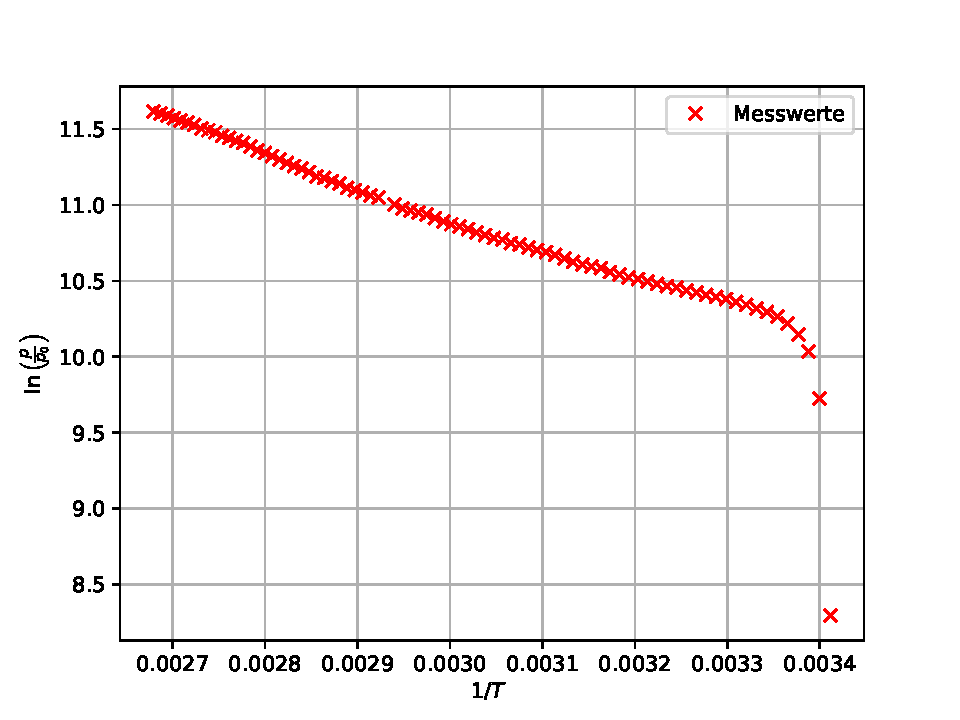
\includegraphics[height=6cm]{plota.pdf}  
    \caption{Bereich von $30$ bis $1000$\,mbar. $p_0=1$/\,mbar.}
    \label{fig:MesswerteKlein}
  \end{subfigure}
  \hfill
  \begin{subfigure}{0.48\textwidth}
    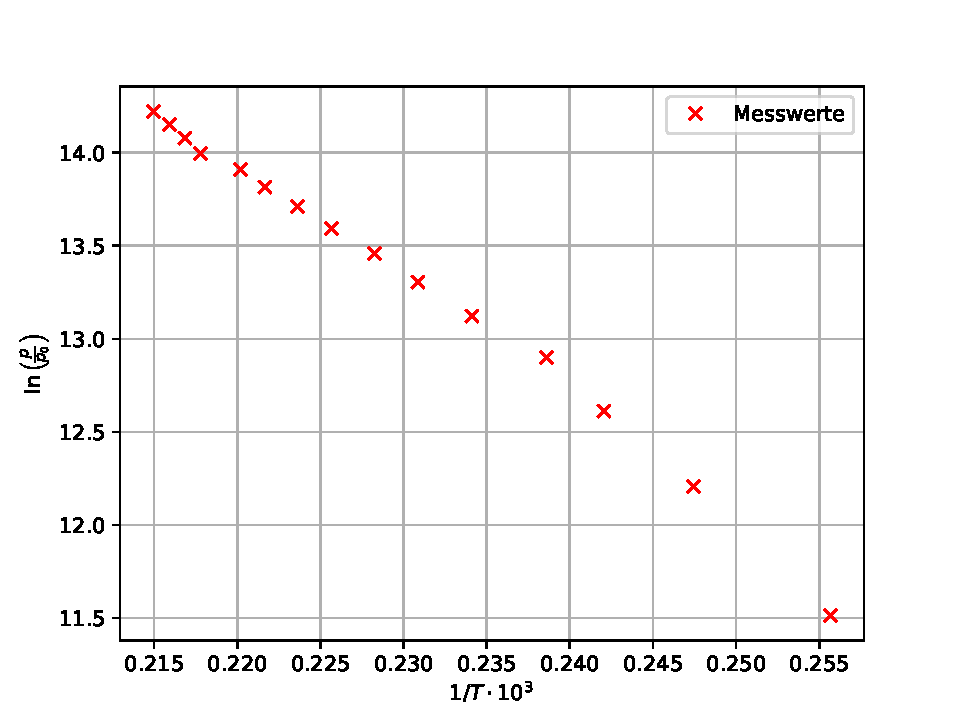
\includegraphics[height=6cm]{plotb.pdf}
    \caption{Bereich von $1$ bis $15 \unit{\bar}$. $p_0=1$/\,bar}
    \label{fig:MesswerteGross}
  \end{subfigure}
  \caption{Die Messwerte der ersten Messreihe aufgetragen als der Logarithmus des Drucks $p$
  gegen die reziproke absolute Temperatur $T$.}
  \label{fig:Teila}
\end{figure}
Um daraus die zu berechnende Verdampfungswärme des Wassers zu bestimmen, wird eine Gerade durch die Messwerte gelegt.
Diese wird mittels Python für den Bereich von $30$ bis $1000$\,mbar erstellt und sieht folgendermaßen aus: \\
\begin{figure}[H]
  \centering
  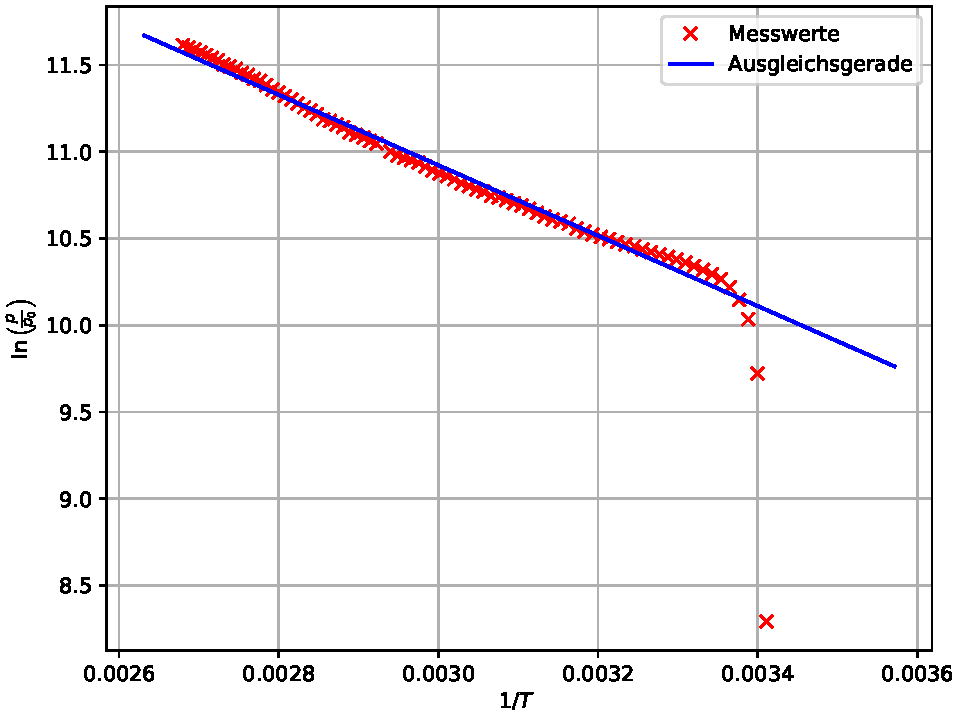
\includegraphics[scale=0.5]{plotc.pdf}
  \caption{Die Messwerte der zweiten Messreihe aufgetragen als der Logarithmus des Drucks $p$
  gegen die reziproke absolute Temperatur $T$ mit der Ausgleichsgerade. $p_0=1$\,mbar.}
  \label{fig:Ausgleichsgerade}
\end{figure}
\newpage
Für diesen Fit wurden die ersten zwei Messwerte dieser Reihe nicht berücksichtigt, da diese die Bestimmung von $L$
offensichtlich verfälschen würden.
Die Gleichung zur Bestimmung von $L$ und dem damit einhergehenden Fit ist wie folgt:
\begin{equation}
  ln(p) = - \frac{L}{R} \cdot \frac{1}{T}
  \Rightarrow y = a \cdot x + b = -2029 * x + 17.010
\end{equation}
Mit numeric Python ergeben sich folgende Messunsicherheiten: $a = \SI{-2029 \pm 21 }{\frac{1}{\kelvin}}$
und $b = \SI{17.010 \pm 0.063}{\frac{1}{\kelvin}}$.
DIe Verdampfungswärme wir mit folgendem Wert und Fehler berechnet:
\begin{equation*}
  L = - \ a \cdot R \Rightarrow L = \SI{16870.1 \pm 174.6}{\frac{\J}{\mol}}
\end{equation*}
L ist die Steigung der Ausgleichsgeraden in Abbildung \ref{fig:Ausgleichsgerade} multipliziert mit der Universellen Gaskonstante R.

Nun folgt die Bestimmung der äußeren Verdampfungswärme $L_a$.
Diese beschreibt die benötigte Arbeit, um bei konstantem Druck das Volumen eines Stoffs zu verändern.
Hierfür wird die ideale Gasgleichung mit der verrichteten Arbeit gleich gesetzt.
\begin{equation}
    W = P \cdot V = R \cdot T = L_a
\end{equation}
Also ergibt sich $L_a = \SI{3101.3}{\frac{\J}{\mol}}$.
Um jetzt noch die erforderliche Arbeit zu Überwindung der molekularen Anziehungskraft bei Verdampfung $L_i$ zu bestimmen, wird
    die Differenz zwischen $L$ und $L_a$ gebildet.
\begin{equation}
    L_i = L - L_a \Rightarrow L_i = \SI{13768.8 \pm 174.6}{\frac{\J}{\mol}}
\end{equation}

\subsection{Druck über einem Bar}
Auflösen er Clausius-Clapeyronschen Gleichung nach $L$ zur Bestimmung der Wärmeabhängigkeit.\\
\begin{align}
  &(V_D-V_F)dp=\frac{L}{T}dT\nonumber\\
  \Leftrightarrow L=&(V_D-V_F)\frac{dp}{dT}T
\end{align}
Errechnet man mittels Python und scipy einen polynomialen Fit dritten Grades, erhält das Polynom $ax^3+bx^2+cx+d$ folgende Werte:
\begin{align*}
  a = 0.020709167025828 ± 0.005971965168968\\
  b = -24.652993974197063 ± 7.691549806645858\\
  c = 9879.126807499247661 ± 3297.004781181593444\\
  d = -1330791.268963911104947 ± 470353.071982218127232\\
\end{align*}
\begin{figure}[h]
\centering
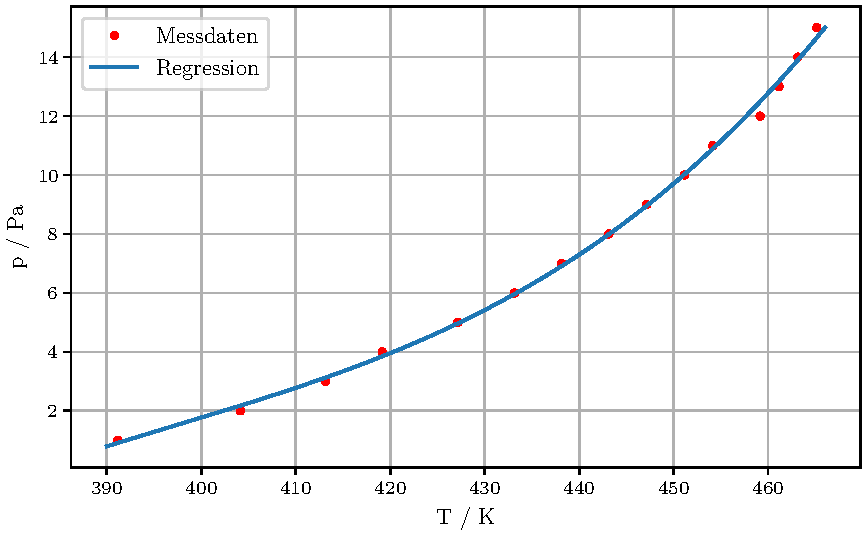
\includegraphics[height=7cm]{plotd.pdf}
\caption{Druck und Temperatur der zweiten Messreihe, $p\geq 1$Bar.}
\label{fig:Druck_groß}
\end{figure}
\\
Ableitung des Polynoms
\begin{equation}
p'(T)=3\cdot a\cdot T^2+2\cdot b\cdot T+c
\end{equation}
Das ist nun unser Asudruck für $\frac{dp}{dT}$.\\
Nun wird die oben in der Theorie schon aufgestellte Annahme genutzt, dass $V_F$ gegen $V_D$
vernachlässigt werden darf. Nach umstellen der Formel aus der Theorie ergibt sich für $V_D$:
\begin{align}
   RT&=\left(p+\frac{a}{V^2}\right)V
   \intertext{wobei. }
   a&=0,9\,\frac{\text{J m}^3}{\text{mol}^2}\nonumber 
   \intertext{ist. Mithilfe der pq-Formel ergibt sich}
   \Rightarrow V&=\frac{RT}{2p}\pm\sqrt{\left(\frac{RT}{2p}\right)^2+\frac{a}{p}}
   \intertext{Durch einsetzen von Gl.(8) in Gl.(5) lässt sich folgender Ausdruck für L schreiben:}
   L(T)&=\frac{T}{P}\left(\frac{RT}{2}\pm\sqrt{\left(\frac{R^2T^2}{4}\right)-ap}\right)
\end{align}
\newpage
Mit Python geplottet sieht $L(T)$ wie folgt aus:
\begin{figure}
  \begin{subfigure}{0.4\textwidth}
  \centering
  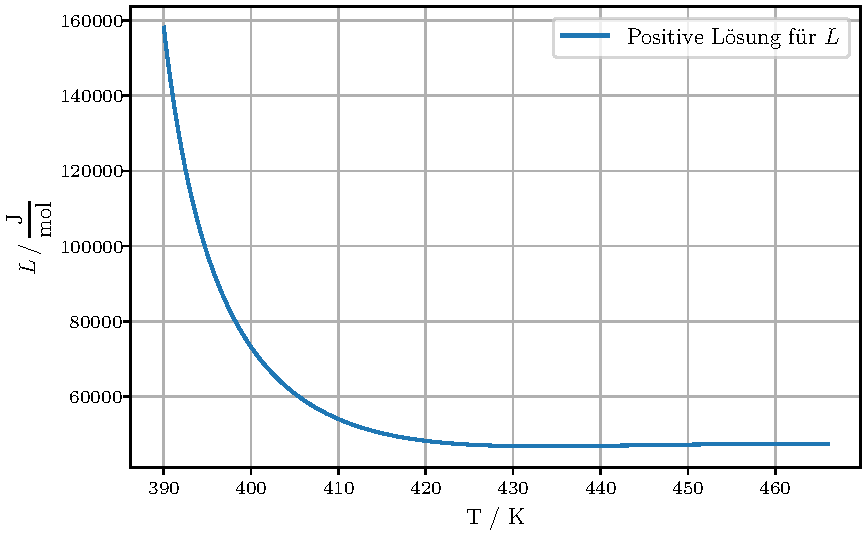
\includegraphics[height=4cm]{plote.pdf}
  \caption{$L$ in Abhängigkeit von T für $V_{D+}$.}
  \label{fig:Verdampfungswärme1}
  \end{subfigure}
  \hfill
  \begin{subfigure}{0.4\textwidth}
  \centering
  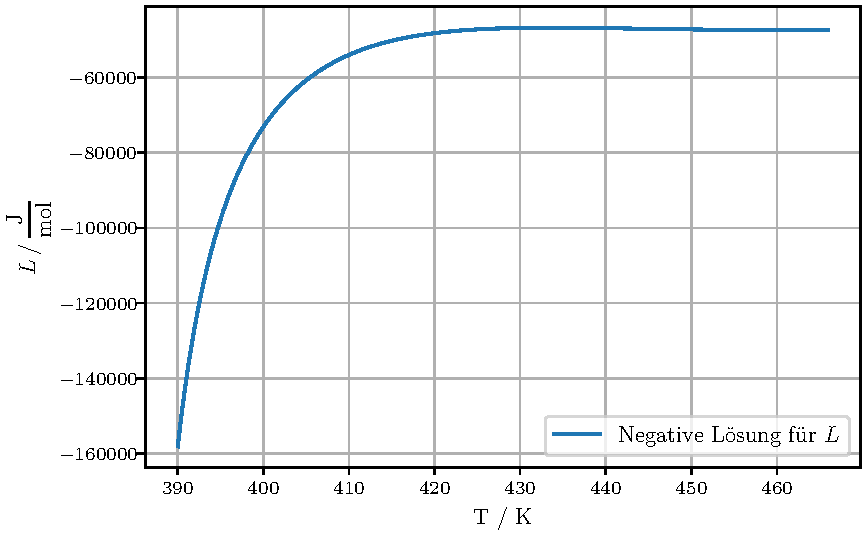
\includegraphics[height=4cm]{plotf.pdf}
  \caption{$L$ in Abhängigkeit von T für $V_{D-}$.}
  \label{fig:Verdampfungswärme2}
  \end{subfigure}
\end{figure}
